% Diagrama da execução em duas fases do CodeMage.
% Compilar dentro do container: xelatex execucao-duas-fases.tex
\documentclass[border=4pt]{standalone}
\usepackage{times}
\usepackage[T1]{fontenc}
\usepackage{tikz}
\usetikzlibrary{positioning,arrows.meta,fit,backgrounds}

\begin{document}
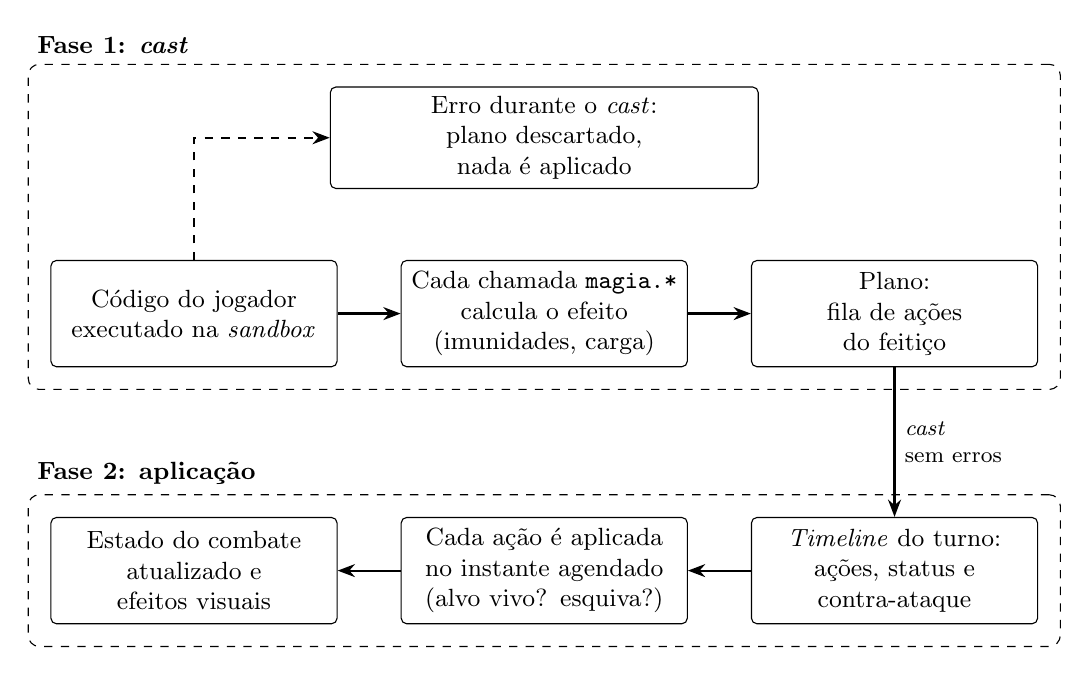
\begin{tikzpicture}[
  font=\small,
  caixa/.style={draw, rounded corners=2pt, align=center, text width=3.4cm,
                minimum height=1.35cm, fill=white},
  seta/.style={-{Stealth[length=2.2mm]}, thick},
  fase/.style={draw, dashed, rounded corners=4pt, inner sep=8pt},
  rotulo/.style={font=\small\bfseries, anchor=south west},
  node distance=0.9cm and 0.8cm
]
  % Fase 1
  \node[caixa] (codigo) {Código do jogador\\executado na \emph{sandbox}};
  \node[caixa, right=of codigo] (api) {Cada chamada \texttt{magia.*}\\calcula o efeito\\(imunidades, carga)};
  \node[caixa, right=of api] (plano) {Plano:\\fila de ações\\do feitiço};

  % Fase 2
  \node[caixa, below=1.9cm of plano] (timeline) {\emph{Timeline} do turno:\\ações, status e\\contra-ataque};
  \node[caixa, left=of timeline] (aplica) {Cada ação é aplicada\\no instante agendado\\(alvo vivo? esquiva?)};
  \node[caixa, left=of aplica] (estado) {Estado do combate\\atualizado e\\efeitos visuais};

  % Erro
  \node[caixa, above=0.9cm of api, text width=5.2cm, minimum height=0.9cm] (erro)
       {Erro durante o \emph{cast}: plano descartado,\\nada é aplicado};

  \draw[seta] (codigo) -- (api);
  \draw[seta] (api) -- (plano);
  \draw[seta] (plano) -- node[right, align=left, font=\footnotesize] {\emph{cast}\\sem erros} (timeline);
  \draw[seta] (timeline) -- (aplica);
  \draw[seta] (aplica) -- (estado);
  \draw[seta, dashed] (codigo.north) |- (erro.west);

  \begin{scope}[on background layer]
    \node[fase, fit=(codigo)(api)(plano)(erro)] (f1) {};
    \node[fase, fit=(estado)(aplica)(timeline)] (f2) {};
  \end{scope}
  \node[rotulo] at (f1.north west) {Fase 1: \emph{cast}};
  \node[rotulo] at (f2.north west) {Fase 2: aplicação};
\end{tikzpicture}
\end{document}
